\chapter*[Cronograma]{Cronograma}
\addcontentsline{toc}{chapter}{Cronograma}

Com o uso da metodologia SCRUM, foram definidas 6 sprints até o fim do projeto. As atividades estão distribuidas, como são mostradas nos gráficos a seguir:


\begin{figure}[p]
	\centering
    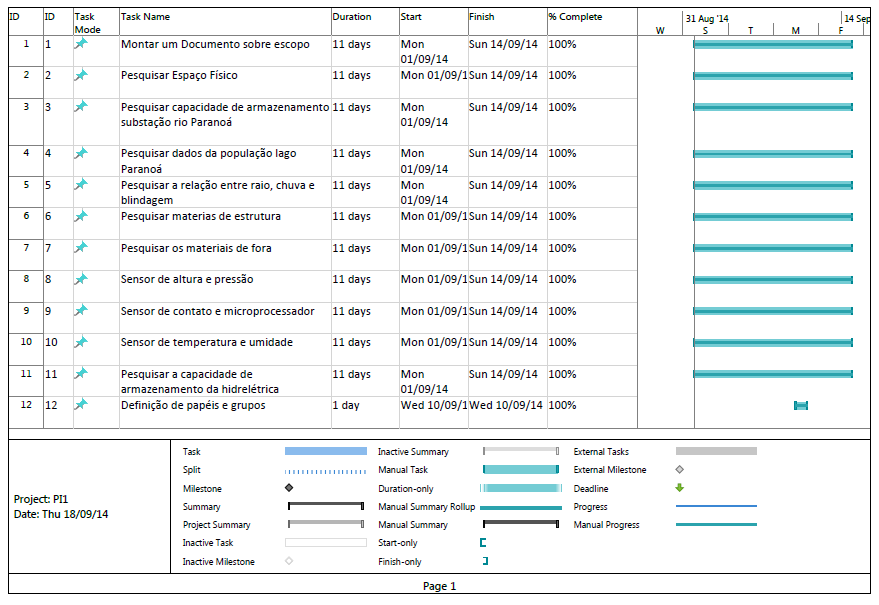
\includegraphics[width=0.8\textwidth]{figuras/sprints1.png}
    \caption{Sprints}
    \label{fig:sprints1}
\end{figure} 

\begin{figure}[p]
	\centering
    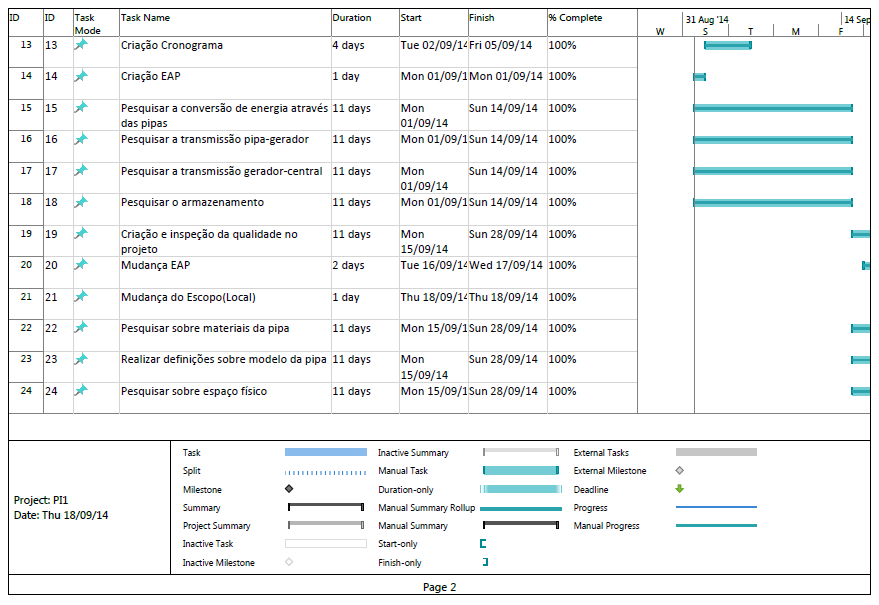
\includegraphics[width=0.8\textwidth]{figuras/sprints2.png}
    \caption{Sprints}
    \label{fig:sprints2}
\end{figure} 


\begin{figure}[p]
	\centering
    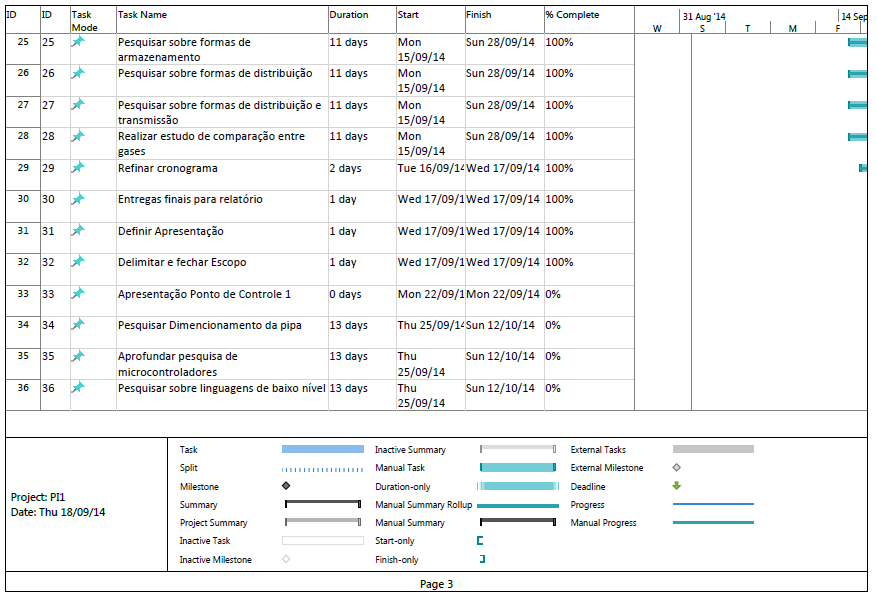
\includegraphics[width=0.8\textwidth]{figuras/sprints3.png}
    \caption{Sprints}
    \label{fig:sprints3}
\end{figure} 